\chapter{Conclusions and Future Work}
This chapter is dedicated to drawing conclusions based on results found and make recommendation on future iterations of this project. Since the underlying methodology is quite novel this system should serve as the foundational step to a fully automated motion capture system.

\section{Conclusion}
The aim of this project was threefold: design a novel wearable data capture system using cameras and sensors to record various parameters of a running bipedal subject, develop a kinematic model to interpret the gathered data points, and design an estimation algorithm to process the captured data. These goals were achieved within certain constraints as discussed in the results section

Due to the relatively small dataset used in this project it serves as a proof of concept and a foundational work that can be iteratively improved.

\section{Future work}
The system was originally designed with four cameras due to the availability of equipment and the assumption that stereo vision would be implemented. From this a set of front and rear mounted cameras would be necessary. Originally there was an intention to reduce the total amount of cameras.

The iterative design would have followed the following mapping. Initially using 4 cameras and an smartphone as a sensor. reducing the system to two cameras (one mounted to the back of the runner and one mounted to the chest of the runner) and a smartphone as a sensor. The next iteration would use the the smartphone camera at the front and a single camera at the back whilst using the smartphone as a sensor as well. This system greatly reduces the cost of the original design philosophy, even given that a powerful and modern smartphone would be used. The final iteration would use only the smartphone at the front as a single camera and sensor. For this method to work the estimation algorithm would need to better understand the periodic motion of the human gait and the model would need to increase in complexity.

Due to the labour intensive approach taken to image processing a further avenue for improvement is the automation of feature detection. The progression would start from the current implementation of markers and use a semi-automatic toolbox to identify critical points on the image. Next computer algorithms should be created to automate the image processing with markers. This could allow for much longer runs and larger datasets to be studied, introducing elements such as fatigue and other running modifiers. The next iterative step would be to remove the markers from the runner such that the setup time of the system is reduces. This is a difficult problem to solve using classical image processing as the variables relating to the runner and the environment are not constant. Perhaps a neural network can be trained to identify the different elements of the lower limbs.

These improvements would decrease the overall cost of the system and optimize the the process substantially. This decrease in hardware does imply that the complexity of the underlying algorithms and models would increase. This trade-off can be considered for future work.

Finally the results obtained have not been verified. An experiment to verify these results was designed, where external cameras would generate three dimensional position data of the markers. This can be compared to the data generated from the EKF as applied to the wearable motion capture system.

\newpage
\begin{figure}[!ht] 
\captionsetup{width=1\linewidth, font=small}  
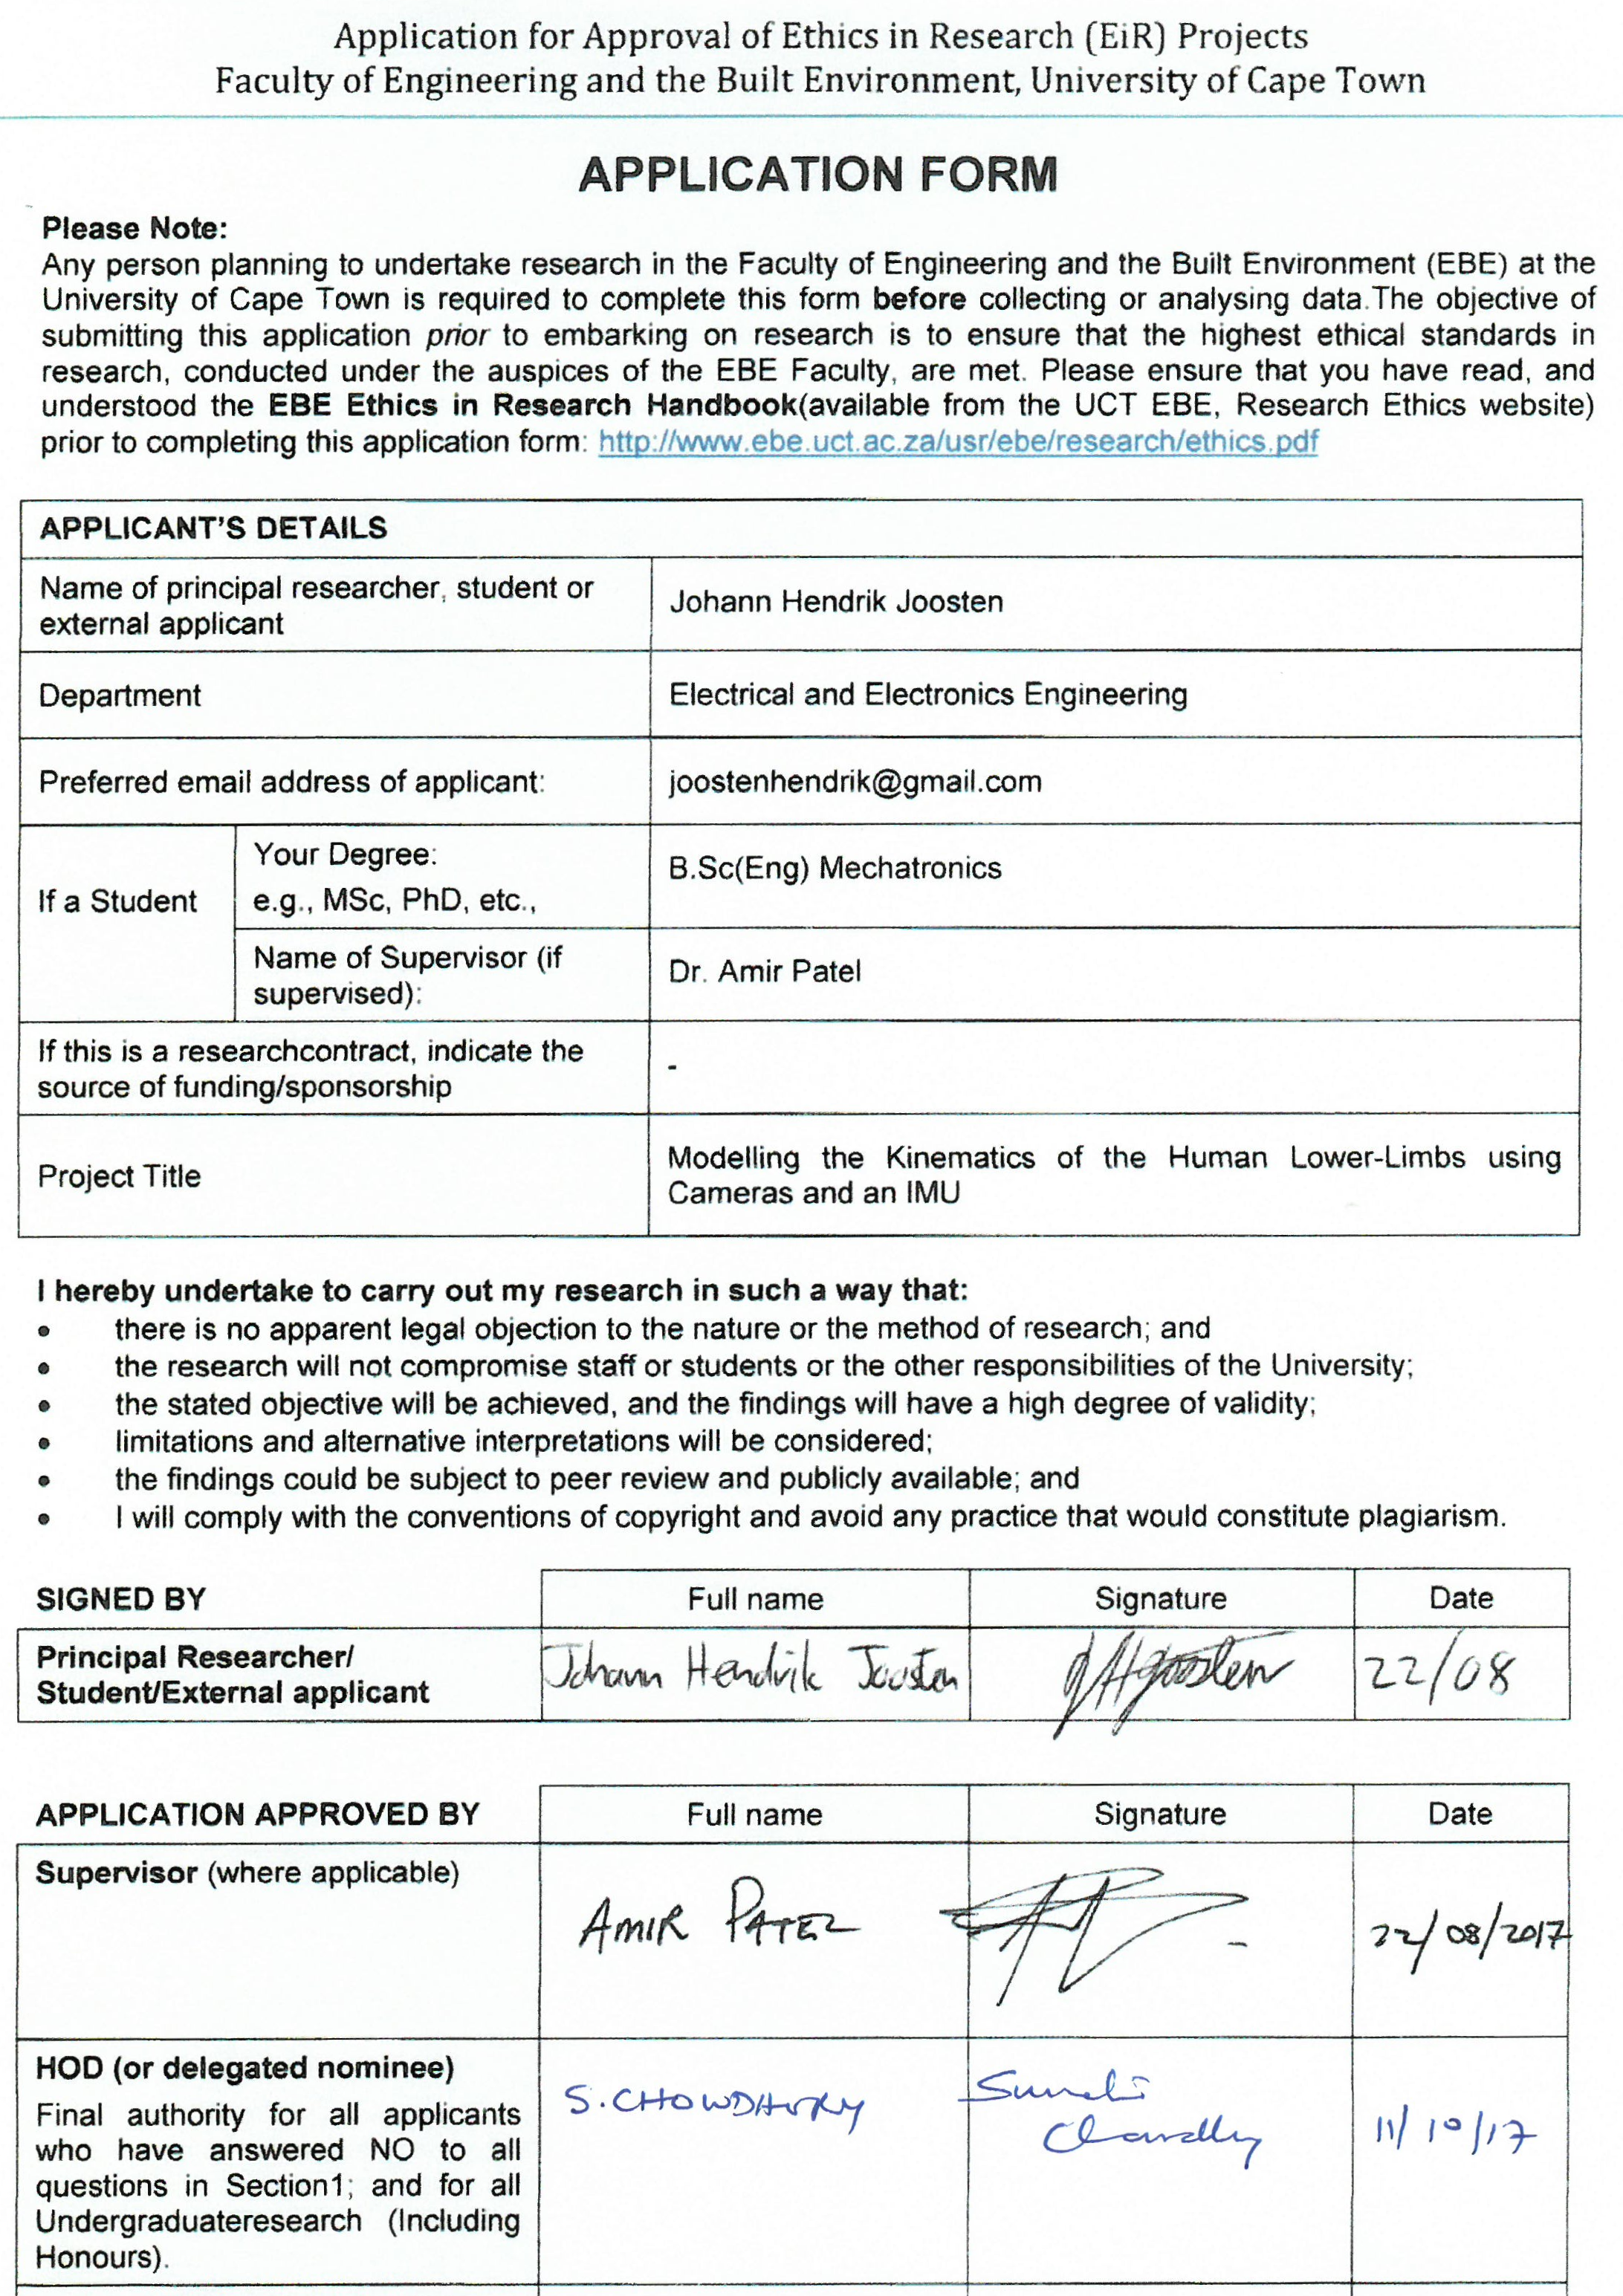
\includegraphics[width=1\linewidth]{figures/ethics.png}
\caption{ethics clearance}
\label{fig:ethics}
\end{figure}








